\section{مقدمه}
\label{sectio:design:preface}
در این فصل از پژوهش روش طراحی منطق دامنه بر اساس تبادل ناهمگام پیغام ارائه شده است. تلاش شده است تا تطابق طراحی با مدل بازیگر در حد امکان حفظ شود. با توجه به تمرکز این بخش بر روش طراحی منطق دامنه و به هدف ایجاد شفافیت و افزایش قابلیت فهم نکات و الگوهای مطرح شده در روش، تصمیم به استفاده از یک سیستم نمونه به عنوان مثال گرفته شد. کلیه‌ی نکات مطرح شده در ادامه‌ی این بخش در قالب این مثال ارائه خواهند شد. در انتخاب سیستم نمونه نکات ذیل مورد توجه قرار گرفته‌ است:
\begin{enumerate}
\item \textbf{دامنه‌ی سیستم انتخابی:}
رده‌ی دامنه‌ی سیستم انتخاب شده به طور کلی سیستم‌های اطلاعاتی\LTRfootnote{informatiion system} است. اولین دلیل انتخاب این رده این است که در این نوع دامنه همروندی به طور ذاتی وجود ندارد و به همین دلیل زمینه‌ی مقایسه‌ی طراحی بر اساس تبادل ناهمگام با  طراحی‌های شیءگرای ترتیبی فراهم می‌شود. با توجه به اینکه یکی از موارد مقایسه‌ی این نوع طراحی با طراحی شیءگرای ترتیبی تفاوت کارایی این دو رویکرد است، دامنه‌ی انتخاب شده باید در حالت ترتیبی هم قابلیت اضافه شدن همروندی را داشته باشد. سیستم‌های اطلاعاتی از این حیث نیز انتخاب مناسبی محسوب می‌شوند چرا که در اکثر پیاده‌سازی‌های عملیاتی، علیرغم داشتن طراحی ترتیبی، به وسیله‌ی ریسمان‌هایی که وب‌سرورها برای پاسخگویی به درخواست‌های همزمان کاربران ایجاد می‌کنند، دارای خاصیت همروندی نیز می‌گردند. به همین دلیل در بخش ارزیابی می‌توانیم با شبیه‌سازی عملیات وب‌سرورها، کارایی و نیز تغییرپذیری دو نوع طراحی مذکور را ارزیابی و مقایسه کنیم.
 دلیل دیگر این انتخاب بالا بودن میزان آشنایی جامعه‌ی طراحی شیءگرا با این نوع سیستم‌ها و استفاده‌ی گسترده از این نوع سیستم‌ها می‌باشد. شایان ذکر است که سعی شده است در ارائه‌ی الگوها و نکات استخراج شده از این طراحی بر دامنه‌ی انتخاب شده تکیه‌ نشود. دامنه‌ی سیستم نمونه نیز یک سیستم آموزشی انتخاب شده است. با توجه به اینکه استفاده کنندگان این پژوهش جامعه‌ی دانشگاهی هستند، آشنایی این جامعه با سیستم آموزشی دلیل اصلی انتخاب آن بوده است. 
\item \textbf{ بزرگی منطق دامنه:}
از نظر میزان بزرگی سیستم (تعداد کلاس‌ها و موارد کاربرد\LTRfootnote{use cases})،‌  سعی شده منطق حد اقل بزرگی و پیچیدگی را داشته باشد تا ضمن امکان مشاهده‌ی الگوهای مختلف، نیازی به تکرار نکات طراحی برای مولفه‌های متعدد و مشابه نباشد. 
\end{enumerate} 

\section{معرفی یک سیستم آموزش ساده }
\label{section:eduIntro}
همان‌طور که در بخش \ref{sectio:design:preface} ذکر شد،‌ یک سیستم آموزش کوچک به عنوان مدل طراحی انتخاب شده است. در ادامه‌ی این بخش ابتدا موارد کاربرد\LTRfootnote{use cases} انتخاب شده در این سیستم را توصیف می‌کنیم و سپس با توجه به‌ آنها مدل دامنه\LTRfootnote{Domain Model} سیستم را در قالب نمودار کلاس بیان می‌کنیم.

\subsection{موارد کاربرد}
در این بخش موارد کاربرد انتخاب شده برای سیستم آموزش معرفی می‌شوند. لازم به تأکید است که علیرغم این که این موارد کاربرد، مرتبط و هماهنگ با موارد کاربرد یک سیستم آموزش واقعی هستند، به هیچ عنوان تمام موارد کاربرد مورد نیاز برای ساختن سیستم واقعی را شامل نمی‌شوند و علاوه‌ بر آن، موارد انتخاب شده دارای جزئیات و دقت کافی برای پوشش فرایند‌های واقعی نیستند. در ادامه‌ی این بخش، هر \gls{مورد کاربرد} در قالب یک جدول توصیفی ارائه شده‌ است.


%%%%%%%%%%%%%%%%%%%%%%%%%%%%%
%%%%  GPA
%%%%%%%%%%%%%%%%%%%%%%%%%%%%%
\begin{table}
\begin{center}
\begin{tabular}{|p{5cm}|p{10cm}|}
	\hline
	\textbf{نام مورد کاربرد} &
درخواست محاسبه‌ی معدل ترم دانشجو\\
	\hline
	\textbf{بازیگر(ان)} &
کاربر\\
	\hline
	\textbf{شروع می‌شود زمانی که} &
درخواست محاسبه‌ی معدل ترم وارد سیستم می‌شود.\\
	\hline
	\textbf{پیش‌شرط‌ها} &
دانشجو و ترم در سیستم تعریف شده باشند.\\
	\hline
	\textbf{جریان اصلی} &
۱. درخواست محاسبه‌ی معدل دانشجو در ترم مربوطه وارد سیستم می‌شود.\newline
۲. سیستم سوابق تحصیلی دانشجو در ترم مربوطه را بررسی ‌می‌کند. معدل ترم با توجه به نمرات اخذ شده و تعداد واحد هر درس محاسبه و اعلام می‌شود. در صورتی که نمره‌ی درس سابقه‌ای وارد نشده باشد، درس مربوطه در محاسبه‌ی معدل لحاظ نمی‌گردد.\\
	\hline
\textbf{جریان استثنا ۱} &
۱.الف) در صورتی که دانشجو هیچ واحدی در ترم جاری اخذ نکرده باشد پیغام خطای مناسب صادر می‌شود و جریان اصلی خاتمه می‌یابد.\\
	\hline
%	\textbf{جریان استثنا ۲} &
%۴-ج. رمز وارد شده نامعتبر است، پیام خطای رمز نامعتبر است به کاربر نمایش داده شده و تراکنش متوقف می‌شود\\
%	\hline
	\textbf{تمام می‌شود زمانی که} &
معدل دانشجو اعلام می‌شود یا خطای مناسب صادر می‌گردد.\\
	\hline
%	\textbf{پس شرط‌ها} &
%کاربر موجودی کارت و یا خطای تراکنش را مشاهده کرده است.\\
%	\hline
\end{tabular}
\caption{\label{table:uc_gpa} توصیف مورد کاربرد محاسبه‌ی معدل یک دانشجو در یک ترم}
\end{center}
\end{table}

%%%%%%%%%%%%%%%%%%%%%%%%%%%%%
%%%%  Take Course
%%%%%%%%%%%%%%%%%%%%%%%%%%%%%
\begin{table}
\begin{center}
\begin{tabular}{|p{4cm}|p{12cm}|}
	\hline
	\textbf{نام مورد کاربرد} &
درخواست اخذ یک ارائه در یک ترم\\
	\hline
	\textbf{بازیگر(ان)} &
کاربر\\
	\hline
	\textbf{شروع می‌شود زمانی که} &
درخواست محاسبه‌ی معدل ترم وارد سیستم می‌شود.\\
	\hline
	\textbf{پیش‌شرط‌ها} &
۱. ‌انتخاب واحد در ترم امکانپذیر باشد. (رجوع کنید به جداول \ref{table:uc_enableofferings}و\ref{table:uc_disableofferings})\\
	\hline
	\textbf{جریان اصلی} &
۱. سیستم کنترل می‌کند که دانشجو در ترم‌های قبل این درس را نگذرانده باشد.\newline
۲. سیستم کنترل می‌کند که دانشجو در ترم‌ جاری این درس را اخذ نکرده باشد.\newline
۳. سیستم کنترل می‌کند که دانشجو تمام پیش‌نیاز‌های این درس را با موفقیت گذرانده باشد.\newline
۴. سیستم کنترل می‌کند که تعداد واحد‌های اخذ شده توسط دانشجو در این ترم پس از اخذ این درس بیشتر از ۲۰ نشود.\newline
۵. سیستم یک سابقه از ارائه‌ی انتخاب شده برای دانشجو تشکیل می‌دهد و آن را در سوابق دانشجو ثبت می‌کند.\\
	\hline
\textbf{جریان استثنا ۱} &
۱.الف)در صورتی که دانشجو قبلا این درس را گذرانده باشد، خطای ''درس انتخاب شده قبلاً گذرانده شده است`` صادر می‌شود و جریان اصلی خاتمه می‌یابد.\\
	\hline
\textbf{جریان استثنا ۲} &
۲.الف)در صورتی که دانشجو در ترم جاری این درس را اخذ کرده باشد، خطای ''این درس در ترم جاری قبلاً اخذ شده است`` صادر می‌شود و جریان اصلی خاتمه می‌یابد.\\
	\hline
\textbf{جریان استثنا ۳} &
۳.الف)در صورتی که دانشجو یکی از پیش‌نیاز‌های درس‌ را نگذرانده باشد، خطای ''انتخاب بیشتر از ۲۰ واحد در ترم مجاز نمی‌باشد`` صادر می‌شود و جریان اصلی خاتمه می‌یابد.\\
	\hline
\textbf{جریان استثنا ۴} &
۴.الف)در صورتی که تعداد واحد‌های اخذ شده توسط دانشجو در این ترم پس از اخذ این درس بیشتر از ۲۰ شود، خطای ''انتخاب بیشتر از ۲۰ واحد در ترم مجاز نمی‌باشد`` صادر می‌شود و جریان اصلی خاتمه می‌یابد.\\
	\hline
	\textbf{تمام می‌شود زمانی که} &
سابقه‌ی جدید در سوابق دانشجو ثبت می‌شود و یا خطای مناسب صادر می‌گردد.\\
	\hline
\end{tabular}
\caption{\label{table:uc_takecoure} توصیف مورد کاربرد اخذ یک ارائه توسط یک دانشجو در یک ترم}
\end{center}
\end{table}

%%%%%%%%%%%%%%%%%%%%%%%%%%%%%
%%%%  DISABLE_TERM_OFFERINGS
%%%%%%%%%%%%%%%%%%%%%%%%%%%%%
\begin{table}
\begin{center}
\begin{tabular}{|p{5cm}|p{10cm}|}
	\hline
	\textbf{نام مورد کاربرد} &
درخواست غیر فعال کردن ارائه‌های یک ترم برای انتخاب واحد\\
	\hline
	\textbf{بازیگر(ان)} &
کاربر(مدیر سیستم)\\
	\hline
	\textbf{شروع می‌شود زمانی که} &
درخواست غیرفعال کردن ارائه‌های یک ترم وارد سیستم می‌شود.\\
	\hline
	\textbf{پیش‌شرط‌ها} &
 ترم در سیستم تعریف شده باشند.\\
	\hline
	\textbf{جریان اصلی} &
۱. درخواست غیر فعال کردن ارائه‌های یک ترم وارد سیستم می‌شود.\newline
۲.سیستم تمام ارائه‌های یک ترم را غیرفعال می‌کند.\\
	\hline
	\textbf{تمام می‌شود زمانی که} &
تمام ارائه‌های ترم برای انتخاب واحد غیرفعال می‌شوند.\\
	\hline
	\textbf{پس شرط‌ها} &
انتخاب واحد در ترم امکان پذیر نیست.\\
	\hline
\end{tabular}
\caption{\label{table:uc_disableofferings} توصیف مورد کاربرد غیرفعال کردن ارائه‌های یک ترم برای انتخاب واحد}
\end{center}
\end{table}

%%%%%%%%%%%%%%%%%%%%%%%%%%%%%
%%%%  ENABLE_TERM_OFFERINGS
%%%%%%%%%%%%%%%%%%%%%%%%%%%%%
\begin{table}
\begin{center}
\begin{tabular}{|p{5cm}|p{10cm}|}
	\hline
	\textbf{نام مورد کاربرد} &
درخواست فعال کردن ارائه‌های یک ترم برای انتخاب واحد\\
	\hline
	\textbf{بازیگر(ان)} &
کاربر(مدیر سیستم)\\
	\hline
	\textbf{شروع می‌شود زمانی که} &
درخواست فعال کردن ارائه‌های یک ترم وارد سیستم می‌شود.\\
	\hline
	\textbf{پیش‌شرط‌ها} &
 ترم در سیستم تعریف شده باشند.\\
	\hline
	\textbf{جریان اصلی} &
۱. درخواست فعال کردن ارائه‌های یک ترم وارد سیستم می‌شود.\newline
۲.سیستم تمام ارائه‌های یک ترم را فعال می‌کند.\\
	\hline
	\textbf{تمام می‌شود زمانی که} &
تمام ارائه‌های ترم برای انتخاب واحدفعال می‌شوند.\\
	\hline
	\textbf{پس شرط‌ها} &
انتخاب واحد در ترم امکان پذیر است.\\
	\hline
\end{tabular}
\caption{\label{table:uc_enableofferings} توصیف مورد کاربرد فعال کردن ارائه‌های یک ترم برای انتخاب واحد}
\end{center}
\end{table}


\subsection{موجودیت‌های اصلی}
\label{subsec:mainEntities}
 موجودیت‌های اصلی  مدل ابتدایی این سیستم عبارتند از:
\textbf{\textit{دانشجو}}\LTRfootnote{Student}، \textbf{\textit{درس}}\LTRfootnote{Course}، \textbf{\textit{ترم}}\LTRfootnote{Term}، \textbf{\textit{ارائه}}\LTRfootnote{Offering} و \textbf{\textit{سابقه}}\LTRfootnote{Study Record}.\\
در هر \textit{ترم} تحصیلی، تعدادی \textit{ارائه} از دروس مختلف وجود دارد. هر درس می‌تواند \textit{ارائه}های مختلفی داشته باشد. به عنوان مثال درس ریاضی۱ می‌تواند در ترم ۹۰-۹۱-۱سه ارائه‌ی مختلف داشته باشد. دانشجو با اخذ هر ارائه \textit{سابقه}‌ای از آن ارائه را به اسم خود ثبت می‌کند. در این سابقه اطلاعاتی مثل نمره‌ی دانشجو و وضعیت قبول یا مردودی درس در طول ترم ثبت خواهد شد. دروس می‌توانند رابطه‌ی پیش‌نیازی\LTRfootnote{prerequisite} باهم داشته باشند. 
\begin{figure*}
    \begin{center}
	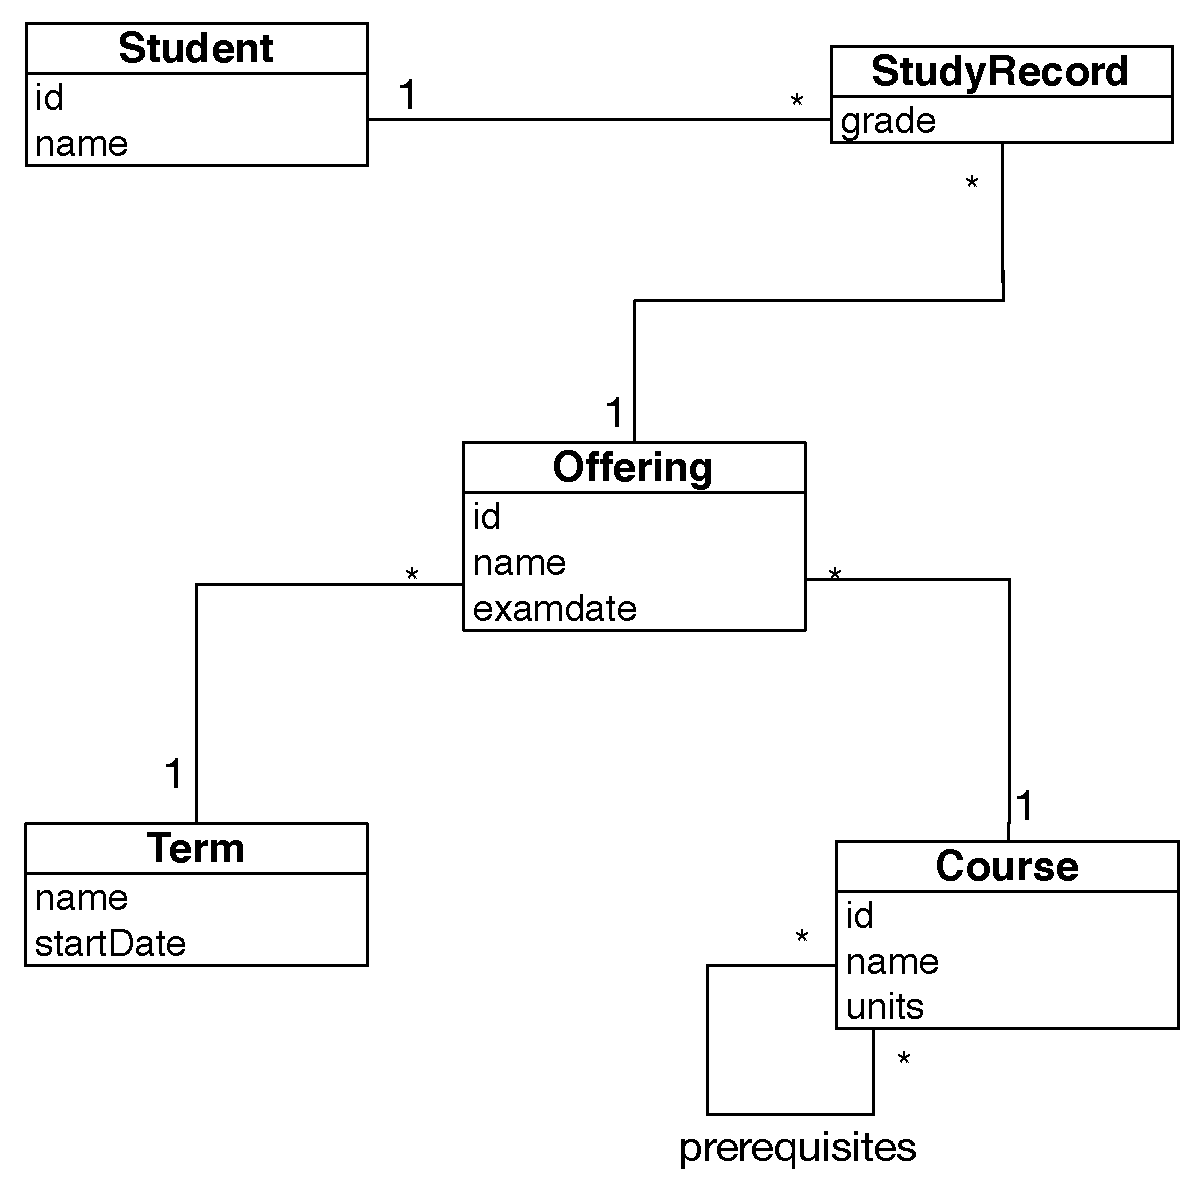
\includegraphics[width=16cm]{4-ProposedFramework/Figures/SimpleClassDiagram.pdf}
    \end{center}
    \caption{\label{fig:edu_class1} نمودار کلاس مدل ابتدای سیستم آموزش ساده }
\end{figure*}
شکل \ref{fig:edu_class1} مدل دامنه‌ی سیستم را به وسیله‌ی یک نمودار کلاس مبتنی بر \textbf{یو‌ام‌ال}\LTRfootnote{UML} نشان می‌دهد.

\newpage
\section{طراحی سیستم آموزش به روش تبادل ناهمگام پیغام}
در این بخش طراحی سیستم معرفی شده در بخش \ref{section:eduIntro} به روش تبادل ناهمگام پیغام ارائه می‌گردد. سعی شده است تا به جای ارائه‌ی یکباره‌ی طراحی نهایی، یک رویکرد \gls{افزایشی}\LTRfootnote{incremental} برای طراحی اتخاذ شود. در این رویکرد مراحل تشکیل نهایی طرح و حتی اقدامات اشتباهی که در طول طراحی برداشته شده است ارائه خواهد شد. به  این ترتیب علاوه بر قابل استفاده‌تر بودن پژوهش به صورت یک دستورالعمل \LTRfootnote{receipe} طراحی، قابلیت فهم روش طراحی هم بالاتر می‌رود.
\subsection{طراحی اکتور‌های اصلی}
منظور از اکتوران اصلی سیستم همان موجودیت‌های اصلی‌ای هستند که در بخش \ref{subsec:mainEntities} معرفی شدند. دلیل استفاده از واژه‌ی \textit{اصلی}  این است که احتمالاً علاوه بر این اکتورها، اکتوران دیگری نیز برای پیاده‌سازی کارکردهای سیستم لازم خواهد شد. در طراحی اکتوران اصلی صرفا فیلد‌های اکتور و نیز پیغام‌های اصلی که از روابط موجود در نمودار کلاس \ref{fig:edu_class1} قابل استخراج هستند در نظر گرفته ‌می‌شود. منطق پیاده‌سازی عملیات هر پیغام و  پیغام‌های دیگری که به این منظور ایجاد می‌شوند در ادامه به طراحی افزوده خواهد شد. 
با توجه به اینکه در مدل اکتور،‌ تنها راه ارتباط بین اکتور‌ها استفاده از تبادل پیغام است و این که یک اکتور برای امکان ارسال پیغام به اکتور دیگر نیاز به دسترسی به اسم آن دارد، بهترین راه برای طراحی رابطه‌های وابستگی\LTRfootnote{association} این است که در کلاس یک اکتور برای هر کلاس دیگر که رابطه‌ای با آن وجود دارد یک فیلد از نوع کلاس طرف دیگر در نظر گرفته شود. این مورد مشابه طراحی شیءگرای عادی (ترتیبی) است. از طرف دیگر در مدل طراحی شیءگرای ترتیبی برای هر کارکرد اصلی یک شیء نیز یک متد در کلاس متناظر با آن در نظر گرفته می‌شود که برای اجرای کارکرد، متد مورد نظر فراخوانی می‌شود. با توجه به اینکه در مدل اکتور مکانیزم کنترلی برنامه به جای فراخوانی متد، تبادل پیغام است، باید به ازای هر متد متناظر در حالت شیءگرا، یک پیغام دریافت شود. البته در این مرحله از طراحی منطق پیاده‌سازی کارکرد هر پیغام در نظر گرفته نشده است و در مراحل بعدی به تدریج اضافه خواهد شد.
\begin{enumerate}
\item\textbf{اکتور دانشجو}\\
اکتور دانشجو دارای فیلد‌های نام و شناسه است. به علت ارتباط دانشجو با سابقه‌ها و نیاز  به ارسال پیغام به آنها یک فیلد از نوع لیست سابقه نیز در کلاس دانشجو وجود دارد. قطعه کد \ref{fig:mainActors:student} طرح ابتدایی کلاس اکتور دانشجو را نشان می‌دهد. همان‌طور که در بخش قبل ذکر شد منطق پیاده‌سازی کارکرد پیغام‌ها در این مرحله اضافه نشده و در ادامه‌ی فصل به تدریج تکمیل خواهد شد. پیغام‌هایی که اکتور دانشجو دریافت می‌کند عبارتند از:
\begin{enumerate}
\item\textbf{:\ltr{HasPassed(course)}}
با دریافت این پیغام اکتور دانشجو باید پاسخ بدهد که آیا درس مربوطه را گذرانده است یا خیر.
\item\textbf{:\ltr{HasTaken(course)}}
با دریافت این پیغام دانشجو باید پاسخ دهد که در ترم جاری این درس را اخذ کرده است یا خیر.
\item\textbf{:\ltr{GPARequest(term)}}
با دریافت این پیغام دانشجو باید پاسخ دهد که معدل دانشجو در ترم جاری  چند بوده است.
\item\textbf{:\ltr{TakeCourse(offering)}}
با دریافت این پیغام دانشجو باید درس ارائه‌ی مربوطه را اخذ کند. طبیعتاً تمام شرایط ذکر شده در مورد کاربرد \ref{table:uc_takecoure} باید بررسی شود.
\end{enumerate}
\codelisting[language=scala]{4-ProposedFramework/src/mainActors/Student.scala}{ساختار کلاس اکتور دانشجو}{fig:mainActors:student}




\end{enumerate}
\subsection{مورد کاربرد ۱}
سلام
\subsubsection{رویکرد اول}
سلام
\subsubsection{رویکرد دوم}
سلام
\subsubsection{رویکرد نهایی}
سلام
\subsection{مورد کاربرد ۲}
سلام

\section{الگوهای طراحی استخراج شده و نکات مهم}
اینجا یه سری الگو می‌دم و رفرنس می‌دم که اینجا اینو دیدیم.
